\documentclass[twoside]{report}

% Use so that < and > get formatted correctly when printed in text
%\usepackage[T1]{fontenc}
\usepackage{acronym}
\usepackage{amsmath}
\usepackage{amssymb}
%\usepackage{array}
\usepackage[blocks]{authblk}
%\usepackage{booktabs}
%\usepackage[toc]{appendix}
%\usepackage{breqn}
\usepackage[justification=justified,singlelinecheck=off,bf]{caption}
\usepackage{chngcntr}
\usepackage{changepage}
\usepackage[usenames,dvipsnames]{color}
\usepackage{enumerate}
\usepackage{enumitem}
\usepackage{fancyhdr}
%\usepackage[Glenn]{fncychap}
\usepackage{fancybox}
\usepackage{fancyvrb}
\usepackage{float}
%\usepackage{framed}
%\usepackage{fullpage}
%\usepackage{gensymb}
\usepackage[top=1.0in,bottom=1.0in,inner=1.0in,outer=1.0in]{geometry}
\usepackage{graphicx}
\usepackage{lastpage}
%\usepackage{listing}
%\usepackage{lscape}
%\usepackage{makecell}
\usepackage{multirow}
%\usepackage{pdflscape}
\usepackage{units}
\usepackage{newfloat}
\usepackage{wrapfig}
%\usepackage{nicefrac}
%\usepackage{multicol}
%\usepackage{xr-hyper}
\usepackage{hyperref}
\usepackage{tabularx}
\usepackage{siunitx}
\usepackage{textcomp}
\usepackage[pages=some]{background}
\usepackage{longtable}
\usepackage{booktabs}
\usepackage{titlesec}

\title{THOR Developer's Manual (NOT YET CONSIDERED RELEASED!)}
\newcommand{\subtitle}{}
\newcommand{\shortTitle}{THOR Developer's Manual}
\author[1]{Nicholas Herring}
\author[1]{Yousry Azmy}
\author[2]{Sebastian Schunert}
\author[3]{Raffi Yessayan}
\author[4]{Rodolfo Ferrer}

\affil[1]{North Carolina State University}
\affil[2]{Idaho National Laboratory}
\affil[3]{Los Alamos National Laboratory}
\affil[4]{Studsvik Scandpower}

\newcommand{\publicationDate}{09/07/2022}


%customize hyperref
%uncomment to underline the hyperlinks in the document
\hypersetup{
        colorlinks,
%	colorlinks=false,
%	pdfborderstyle={/S/U/W 1},
%	pdfborder=0 0 1,
	linkcolor=black,
	citecolor=black,
	}


% Make custom blue to match word blue
\definecolor{DocNameRed}{RGB}{206,32,41}
% CASL blue
\definecolor{NCSURed}{RGB}{206,32,41}
\definecolor{TitleRed}{RGB}{204,0,2}


% All the other pages style
\renewcommand{\headrulewidth}{0pt}
\fancyhead{}
\fancyfoot{}
\fancyhead[LO,RE]{
\includegraphics[width=1.15in]{../template/NCSU_logo.png}}
\fancyhead[RO,LE]{\color{white}\shortTitle}
\fancyfoot[LE,RO]{\textcolor{NCSURed}{NCSU} Radiation Transport Group}
\fancyfoot[CO,CE]{\thepage}

\fancypagestyle{plain}
{
\fancyhead[LO,RE]{
\includegraphics[width=1.15in]{../template/NCSU_logo.png}}
\fancyhead[RO,LE]{\color{NCSURed}\shortTitle}
\fancyfoot[LE,RO]{\textcolor{NCSURed}{NCSU} Radiation Transport Group}
\fancyfoot[CO,CE]{\thepage}
}

% The title page style
\fancypagestyle{firststyle}
{
   \fancyhead[L]{}
   \fancyfoot[]{}
}


\backgroundsetup{
scale=1,
color=black,
opacity=1.0,
angle=0,
contents={%
  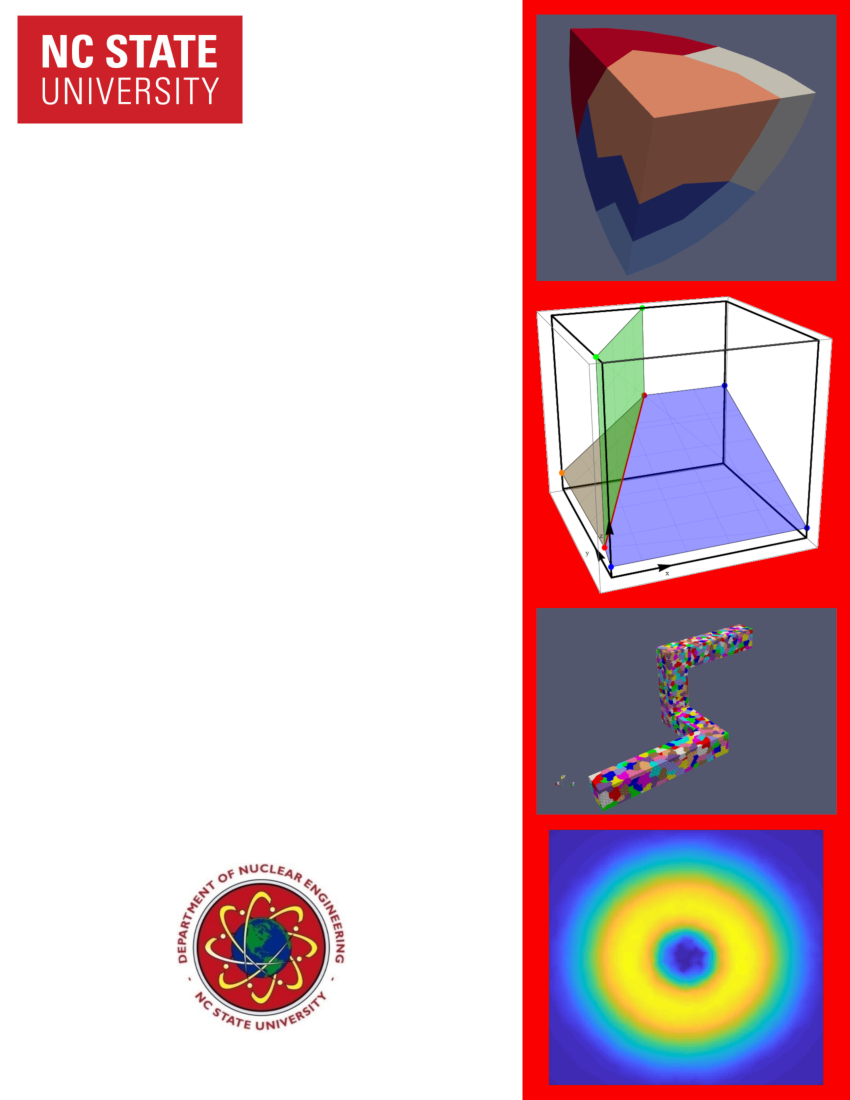
\includegraphics[width=\paperwidth,height=\paperheight]{../template/NCSU_background.pdf}
  }%
}

% Define command to surround text in angle brackets
\newcommand{\brackets}[1]{\textlangle{}#1\textrangle{}}

% For formatting code
\newcommand{\codeblock}[1]{\texttt{#1}}

%increase space after captions
\setlength{\belowcaptionskip}{2pt}

% No indenting at start of paragraph
\setlength{\parindent}{0pt}

%increase space between paragraphs
\parskip 1em

\titleformat{\chapter}{\Huge\bfseries}{\thechapter. }{0pt}{\Huge\bfseries}

% set the section numbering depth and TOC depth
\setcounter{secnumdepth}{3}
\setcounter{tocdepth}{3}

% Use continuous counting scheme for floats
\counterwithout{table}{chapter}

\let\DeclareUSUnit\DeclareSIUnit
\let\US\SI
\DeclareUSUnit\F{F}
\DeclareUSUnit\ft{ft}

% Set list spacing to zero
%\setitemize{itemsep=0em}

\begin{document}

%clear the header/footer until TOC
\pagenumbering{roman}

\begin{titlepage}

   \BgThispage
   \thispagestyle{firststyle}

   \vspace*{\fill}

   \begin{minipage}[l][][c]{0.6\textwidth}
   \begin{flushleft}
   \makeatletter
   {\huge\color{TitleRed}\bf NC State University - Nuclear Computational \\ Science Group}\\
   \vspace{3cm}
   {\huge\fontfamily{phv}\selectfont\color{TitleRed}\bf
   % Title of the document
   \@title\par
   }
   {\Large\fontfamily{phv}\selectfont\color{DocNameRed}\bf
   \subtitle\par
   }
   \vspace*{30pt}
   % Authors
   {\Large\bf\setlength{\parskip}{10pt}
   \@author

   }
   \vspace*{30pt}
   {\huge\bf
   \publicationDate
   }
   \makeatother


   \end{flushleft}
   \end{minipage}

   \vspace*{\fill}

\vspace{1cm}


   \end{titlepage}

   \pagestyle{fancy}

   \vspace*{\fill}

   \captionsetup{justification=centering}
   \begin{table}[H]
   \centering
   \caption*{\Large\bfseries{Revision Log}}
   \begin{tabular}{rrrr}
   \toprule
   \textbf{Version} & \textbf{Date} & \textbf{Affected Pages} & \textbf{Revision Description} \\
   \midrule
   1.0.0 & 09/07/2022 & All & Initial Release \\
   & & & \\
   & & & \\
   \bottomrule
   \end{tabular}
   \end{table}

   \vspace*{\fill}

   \captionsetup{justification=justified}

   \vspace*{\fill}

% no abstract in users' manual
%\begin{center}
  {\large \bfseries \noindent Abstract}
\end{center}

Add Abstract here  (not part of SMP)

\chapter*{Acronyms}
\begin{acronym}
    \acro{THOR}{\textit{TetraHedral-grid High Order Radiation transport code}}
    \acro{AHOT}{\textit{Arbitrarily High Order Transport}}
    \acro{AHOT-C}{\textit{Arbitrarily High Order Transport method of the Characteristic type}}
    \acro{AHOT-N}{\textit{Arbitrarily High Order Transport method of the Nodal type}}
    \acro{AHOT-C-UG}{\textit{Arbitrarily High Order Transport method of the Characteristic type on Unstructured Grids}}
    \acro{SN}{discrete ordinates}
    \acro{MOC}{\textit{Method of Characteristics}}
    \acro{LC}{\textit{Linear Characteristics}}
    \acro{SC}{\textit{Step Characteristic}}
    \acro{DFEM}{\textit{Discontinuous Finite Element Method}}
    \acro{DGFEM}{\textit{Discontinuous Galerkin Finite Element Method}}
    \acro{ESC}{\textit{Extended Step Characteristics}}
    \acro{SBA}{\textit{Slice Balance Approach}}
    \acro{CT}{\textit{Characteristic Tetrahedron}}
\end{acronym}

% table of contents
\tableofcontents

% list of figures
% \listoffigures

% list of tables
% \listoftables
\clearpage
\pagenumbering{arabic}
\pagestyle{fancy}

\chapter{Call Chart}

\section{Obtaining THOR}

This section describes how to obtain \ac{THOR}.
Please contact the code owner~\href{mailto:yyazmy@ncsu.edu}{Yousry Azmy} to be added to the project's membership.

Once a user has been added to the projects membership, they can navigate to their desired installation directory and clone \ac{THOR} from the \ac{NCSU} GitHub repository using the following command:
\begin{verbatim}
  >> git clone https://github.ncsu.edu/NCSU-Rad-Transport/THOR.git
\end{verbatim}
Alternatively, a user who will communicate frequently with \ac{THOR}'s GitHub repository can link their computer's ssh keys with their GitHub account and clone \ac{THOR} directly by issuing the following command:
\begin{verbatim}
  >> git clone git@github.ncsu.edu:NCSU-Rad-Transport/THOR.git
\end{verbatim}

\section{Obtaining LAPACK dependencies}

\ac{THOR} depends on certain \href{http://www.netlib.org/lapack/}{\ac{LAPACK}} routines.
These are provided with \ac{THOR} as a sub-module.
The \ac{LAPACK} submodule can be initialized by:
\begin{verbatim}
    >> git submodule update --init
\end{verbatim}
The \ac{LAPACK} submodule is not expected to change at all.
However, if it does, the \ac{THOR} repository keeps track of the associated version of the \ac{LAPACK} repository, so the user may run:
\begin{verbatim}
    >> git submodule update
\end{verbatim}
to obtain the latest \ac{LAPACK} submodule.
If as expected \ac{LAPACK} hasn't changed an empty line will be displayed.

\section{Compiling THOR}

This section describes how to compile \ac{THOR} and its dependencies.
The first step is to compile the \ac{LAPACK} dependency.
To this end, navigate to the installation scripts using (where \verb"<thor_dir>" is the directory \ac{THOR} was cloned into):
\begin{verbatim}
    >> cd <thor_dir>/contrib/scripts
\end{verbatim}
Edit the file \verb"make.inc" to specify the MPI Fortran compiler available on the local machine (if {\tt gfortran} and {\tt mpich} are being used, there is no need to make any changes).
Also, if necessary, enter command line that modify the environment to enable the compilation process to find the path to required executables; these typically have the form \verb">> load module pathname", where \verb"pathname" is a directory on the local computer where these necessary executables reside.
Execute the \verb"build_lapack.sh" script by (first command may not be necessary, it only ensures that \verb"build_lapack.sh" is executable):
\begin{verbatim}
    >> chmod +x build_lapack.sh
    >> ./build_lapack.sh <n>
\end{verbatim}
where \verb"<n>" is the number of processors.
%At this point it must be provided even if it is \verb"1".
For example, on Idaho National Laboratory's Sawtooth HPCthe compiler is set in \verb"make.inc" via the statement \verb"FORTRAN = mpif90", and the environment is  modified with the command line
\begin{verbatim}
    >> module load mvapich2/2.3.3-gcc-8.4.0".
\end{verbatim}
A successful \ac{LAPACK} build will conclude the scrolled output on the screen with a table of the form:
\begin{verbatim}
                        -->   LAPACK TESTING SUMMARY  <--
                Processing LAPACK Testing output found in the TESTING directory
SUMMARY                 nb test run     numerical error         other error
================        ===========     =================       ================
REAL                    1291905         0       (0.000%)        0       (0.000%)
DOUBLE PRECISION        1292717         0       (0.000%)        0       (0.000%)
COMPLEX                 749868          0       (0.000%)        0       (0.000%)
COMPLEX16               749588          1       (0.000%)        1       (0.000%)

--> ALL PRECISIONS      4084078         1       (0.000%)        1       (0.000%)
\end{verbatim}
The \ac{LAPACK} build may conclude with:
\begin{verbatim}
make[2]: Leaving directory '<thor_dir>/contrib/lapack/TESTING/EIG'
NEP: Testing Nonsymmetric Eigenvalue Problem routines
./EIG/xeigtstz < nep.in > znep.out 2>&1
make[1]: *** [Makefile:464: znep.out] Error 139
make[1]: Leaving directory '<thor_dir>/contrib/lapack/TESTING'
make: *** [Makefile:43: lapack_testing] Error 2
\end{verbatim}
These errors indicate that the system did not have enough memory allocated to \ac{LAPACK} to complete the entirety of the testing suite.
This is typically not a concern and if these are the sole errors, the user is free to continue on to the next step.
The correctness of \ac{THOR} and the \ac{LAPACK} linkage can later be verified with the regression tests if the user so desires.

Now, \ac{THOR} can be compiled. Navigate to the cloned \ac{THOR} folder, and then to the source folder within it:
\begin{verbatim}
    >> cd \verb"<thor_dir>"/THOR/src
\end{verbatim}
and, as before, edit the file \verb"Makefile" to utilize the available MPI Fortran compiler and if necessary modify the environment to enable \verb"make" to locate the compiler (again, for {\tt gfortran} and {\tt mpich}, no changes are necessary).
Then type:
\begin{verbatim}
    >> make
\end{verbatim}
Successful compilation of \ac{THOR} will conclude with the line:
\begin{verbatim}
    mv ./thor-1.0.exe ../
\end{verbatim}
The \ac{THOR} executable (named in the above line) can be found here:
\begin{verbatim}
    >> ls <thor_dir>/THOR/
\end{verbatim}
that should produce:
\begin{verbatim}
    doc  examples  hello_world  scripts  src   thor-1.0.exe  unit
\end{verbatim}

\section{Running THOR for the first time}

Navigate to the \verb"hello_world" directory:
\begin{verbatim}
    >> cd <thor_dir>/THOR/hello_world
\end{verbatim}
Check the content of this folder:
\begin{verbatim}
    >> ls
\end{verbatim}
It should show the following files:
\begin{verbatim}
    >> ls
    hello_world.in hello_world.o hello_world.thrm hello_world.xs
\end{verbatim}
These files have the following significance:
\begin{itemize}
    \item \verb"hello_world.in" is a sample input file to \ac{THOR}. This file is used to execute \ac{THOR}.
    \item \verb"hello_world.thrm" is the corresponding mesh file that is referenced within \verb"hello_world.in". At this point, it is only important that it is present and has the proper \ac{THOR} mesh format. Creation of \ac{THOR} mesh files is covered later in this manual.
    \item \verb"hello_world.xs" is the corresponding cross section file, also referenced within \verb"hello_world.in", and again at this point, it is only important that it is present.
    \item \verb"hello_world.o" is the corresponding output file created by redirecting \ac{THOR}'s standard output. This file can be used to compare \ac{THOR}'s printed output with what it should be upon correct termination of this run.
\end{itemize}
\ac{THOR} is invoked with the executable name and the standard input file that is specified as the first and only command line argument passed to \ac{THOR}.
\begin{verbatim}
    >> ../thor-1.0.exe hello_world.in
\end{verbatim}
For parallel execution type:
\begin{verbatim}
    >> mpirun -np <n> ../thor-1.0.exe hello_world.in
\end{verbatim}
where \verb"<n>" is the number of processors.
Several files should have been created:
\begin{itemize}
    \item \verb"hello_world.flux"
    \item \verb"hello_world.fluxeven"
    \item \verb"hello_world.fluxodd"
    \item \verb"hello_world.in.log"
    \item \verb"hello_world.in_out.csv"
    \item \verb"intermediate_output_even.dat"
    \item \verb"intermediate_output_odd.dat"
\end{itemize}
The significance of these files will be discussed later.
\ac{THOR}'s standard output should start with a banner and conclude with:
\begin{verbatim}
--------------------------------------------------------
   Region averaged reaction rates
--------------------------------------------------------

-- Region --   0 Volume=   1.500000E+01
   Group          Flux       Fission    Absorption      Fiss Src
       1  9.515584E-01  1.284604E+00  8.564026E-01  1.284604E+00
   Total  9.515584E-01  1.284604E+00  8.564026E-01  1.284604E+00


--------------------------------------------------------
   Execution of THOR completed successfully
--------------------------------------------------------
\end{verbatim}

\subsection{Running THOR Regression Tests}

If \ac{THOR} appears to be running properly, it is recommended that the user run \ac{THOR}'s regression tests after making \ac{THOR}.
To do this, navigate to the regression tests directory:
\begin{verbatim}
    >> cd <thor_dir>/THOR/examples/regression_tests
\end{verbatim}
and run the script to run all regression tests
\begin{verbatim}
    >> bash ./runall.bash <n>
\end{verbatim}
Here \verb"<n>" is the number of processors to use (default 1).
These tests will take some time.
For 24 threads, these tests take about 2 to 3 hours.
As such, it is recommended that this testing be performed overnight.
It should also be noted that two of the inputs, \verb"homogeneous_cube_keig_1G/keig_jfnk.inp" and \verb"takeda-IV/takeda_jfnk.inp", use JFNK in problems with opposing reflective boundary conditions.
\ac{THOR} currently does not support the running of such problems in parallel.
As such the user should manually rerun those problems after the testing script completes unless the user originally specified \verb"<n>"=1.

\section{Pre/post Processors}

\subsection{Mesh Converter}\label{ch:getstart:sec:preproc:subsec:meshconv}

The mesh converter is the current recommended pre-processessing utility for \ac{THOR} meshes.
This converter takes a version 4 \href{https://gmsh.info/}{Gmsh} file (tested with version 4.1) and converts it to the \ac{THOR} mesh input file described in Section~\ref{ch:inp:sec:meshfile}.
There are plans to extend this converter to intake other versions of Gmsh and exodus and even perhaps add other output formats in addition to the current \ac{THOR} mesh output.
As of the publishing of this manual, Gmsh version 4.1 is the most recent release Gmsh mesh file format.

To compile the Mesh Converter, navigate to the source folder:
\begin{verbatim}
  >> cd <thor_dir>/pre-processors/Mesh_Converter/src
\end{verbatim}
and then make the converter by typing:
\begin{verbatim}
  >> make
\end{verbatim}
A successful compilation of the Mesh Converter will conclude with the line:
\begin{verbatim}
  >> mv ./Mesh_Converter.exe ../
\end{verbatim}
The Mesh Converter does not have any software requirements that are not also required by \ac{THOR}.

To run the Mesh Converter, simply invoke the mesh converter binary and follow it immediately with the Gmsh input file (where \verb"<gmsh_file>" is the name of the Gmsh file):
\begin{verbatim}
  >> <path_to_Mesh_Converter>/Mesh_Converter.exe <gmsh_file>
\end{verbatim}
The output file will be titled \verb"<gmsh_file>_out.thrm".
This output will set all boundary conditions to vacuum.
If the user desires to set boundary conditions to reflective or incoming flux boundary conditions, then boundary conditions can be specified on the command line when invoking the Mesh Converter by using the \verb"-bc" indicator.
If the \verb"-bc" indicator is called, then the next six entries will be assumed to be the boundary conditions (integer values) on each of the six primary directions.
The order for the boundary conditions specified in this manner are as follows:
\begin{verbatim}
 -x +x -y +y -z +z
\end{verbatim}
0 is the integer value for vacuum boundary conditions, 1 is the integer value for reflective boundary conditions, and 2 is the integer value for incident flux boundary conditions.
i.e. The following use of the Mesh Converter will convert the Gmsh file and assign reflective boundary conditions to the $-x$, $-y$, and $+y$ boundary faces, and all other boundary conditions will be set to vacuum.
\begin{verbatim}
  >> <path_to_Mesh_Converter>/Mesh_Converter.exe <gmsh_file> -bc 1 0 1 1 0 0
\end{verbatim}
It should be noted that if reflective boundary conditions are specified, then the reflective boundaries must all reside on flat boundary surfaces.
If the user tries to assign reflective boundary conditions to a direction with a non-flat boundary, then the converter utility will throw an error and terminate.
This check is ignored if all boundary conditions are reflective.

\subsection{Cross Section Converter}\label{ch:getstart:sec:preproc:subsec:xsconv}

The \ac{XS} converter is the current recommended pre-processessing utility for \ac{THOR} cross sections.
This converter takes one of several different input \ac{XS} formats and converts them to one of several different output \ac{XS} formats.

The \ac{XS} converter DOES have software requirements that are not also required by \ac{THOR}, namely the HDF5 developer's tools.
If the user wishes to acquire HDF5 in order to install and use the \ac{XS} converter, they may do so with the command (for deb package managers):
\begin{verbatim}
  >> sudo apt install libhdf5-dev
\end{verbatim}
To compile the \ac{XS} converter, navigate to the source folder:
\begin{verbatim}
  >> cd <thor_dir>/pre-processors/XS_Converter/src
\end{verbatim}
and then make the converter by typing:
\begin{verbatim}
  >> make
\end{verbatim}
A successful compilation of the \ac{XS} converter will conclude with the line:
\begin{verbatim}
  >> mv ./XS_Converter.exe ../
\end{verbatim}

To run the \ac{XS} converter, simply invoke the \ac{XS} converter binary and follow it immediately with the XS input file followed by the XS output format (where \verb"<xs_in>" is the name of the XS input file and \verb"<out_form>" is the output format):
\begin{verbatim}
  >> <path_to_XS_Converter>/XS_Converter.exe <xs_in> <out_form>
\end{verbatim}
The output file will be titled \verb"<xs_in>_<out_form>.out" unless the output is for an HDF5 format (such as OpenMC cross sections), in which case it will be of the form \verb"<xs_in>_<out_form>.out.h5".

Currently, the THOR \ac{XS} converter only supports the following input/output formats:
\begin{itemize}
  \item Input formats:
    \begin{itemize}
      \item \href{https://serpent.vtt.fi/mediawiki/index.php/Description_of_output_files}{Serpent Version 2 multigroup \ac{XS} output}
      \item THOR \ac{XS} format described in Section~\ref{ch:inp:sec:xsfile}
      \item \href{https://docs.openmc.org/en/stable/}{OpenMC} \ac{XS} HDF5 formatted cross sections \href{https://nbviewer.org/github/openmc-dev/openmc-notebooks/blob/main/mgxs-part-i.ipynb}{generated by OpenMC.}
    \end{itemize}
  \item Output formats:
    \begin{itemize}
      \item \verb"THOR" - THOR \ac{XS} format described in Section~\ref{ch:inp:sec:xsfile}
      \item \verb"OpenMC" - Creates an initial \href{https://www.python.org/}{Python} script for running with \href{https://docs.openmc.org/en/stable/}{OpenMC}.
        This script only contains the commands to create and use the cross sections so the user must either add it to an existing OpenMC script, or create one with this initial baseline by adding geometry, settings, etc.
    \end{itemize}
\end{itemize}
There are also plans to add the following formats for input/output as well:
\begin{itemize}
  \item MPACT/VERA - Export controls allowing.
  \item MCNP - Export controls allowing.
\end{itemize}

\subsection{THOR\_MESH\_Generator}

THOR\_MESH\_Generator is an older pre-processor that converts \textit{exodus} and \textit{gmsh} (the legacy version 2) mesh formats to \ac{THOR}'s native mesh format.
It is currently undergoing maintenance and will likely have important capabilities simply added to the Mesh Converter after which it may be removed.
As such, use of the THOR\_MESH\_Generator is not currently recommended.

% TODO: Update THOR MESH generator or add capabilities to the Mesh Converter
% \ac{THOR} mesh generator is an older pre-processor that converts \textit{exodus} and \textit{gmsh} (the legacy version 2) mesh formats to \ac{THOR}'s native mesh format.
% It also permits uniform refinement of meshes provided in exodus files. Conversion from \textit{exodus} format and uniform refinement uses the
% \textit{libmesh}~\cite{libMeshPaper} \textit{meshtool}. Therefore,
% \textit{libmesh} has to be set up first. To this end, navigate to the \verb"scripts" directory:
% \begin{verbatim}
    % >> cd /home/<usr>/projects/THOR/contrib/scripts
% \end{verbatim}
% and execute \verb"build_libmesh.sh":
% \begin{verbatim}
    % >> chmod +x build_libmesh.sh
    % >> ./build_libmesh.sh <n>
% \end{verbatim}
% where the first command makes \verb"build_libmesh.sh" executable (if it is not already) and \verb"<n>" is the number of processors. It must be provided even if it is simply 1. Executing this script may take a long time to complete installing \textit{libmesh}, however, it will show progress on the screen. If the git-clone command in the \verb"build_libmesh.sh" script does not work, replace it with the command:
% \begin{verbatim}
% git clone https://github.com/libMesh/libmesh.git
% \end{verbatim}
% Finally, the \verb"THOR_LIBMESH_DIRECTORY" environment variable has to be set. This environment variable must point to the directory that the \verb"meshtool-opt" executable is located. For the standard installation, one should execute:
% \begin{verbatim}
    % >> export THOR_LIBMESH_DIRECTORY=/home/<usr>/projects/THOR/contrib/libmesh/build
% \end{verbatim}

% The next step is to make the THOR\_MESH\_GENERATOR application. Navigate to its source folder:
% \begin{verbatim}
    % >> cd /home/<usr>/projects/THOR/pre-processors/THOR_Mesh_Generator/src
% \end{verbatim}
% and type:
% \begin{verbatim}
    % >> make
% \end{verbatim}
% The exectutable
% \begin{verbatim}
    % /home/<usr>/projects/THOR/pre-processors/THOR_Mesh_Generator/Thor_Mesh_Generator.exe
% \end{verbatim}
% should have been created.

% \begin{verbatim}
% ***************************************************************
% The tests as described below did not execute as described.
% Instead, I did the following and still execution of the tests
% did not work properly:

% 1. In ~/PROJECTS/THOR/pre-processors/THOR_Mesh_Generator:
% ln -s Thor_Mesh_Generator\_MP.exe Thor_Mesh_Generator.exe

% 2. In ~/PROJECTS/THOR/pre-processors/THOR\_Mesh_Generator/scripts:
% chmode u+x test\_all.sh

% 3. ./test\_all.sh
% This ran but did not give the output below and reported execution
% errors. It is not clear if these reported errors are part of the
% testing since some of the cases are labeled Bad, or the error
% indicates erroneous installation of libmesh.
% ***************************************************************
% \end{verbatim}


% To ensure that the THOR\_MESH\_GENERATOR application compiled correctly, execute the regression tests. Change directory to:
% \begin{verbatim}
    % >> cd /home/<usr>/projects/THOR/pre-processors/THOR_Mesh_Generator/scripts
% \end{verbatim}
% and execute:
% \begin{verbatim}
    % >> python run_thor_tests.py
% \end{verbatim}
% You should see screen output similar to this:
% \begin{verbatim}
% --------------------------------------------------------------------------------
% Test  1 tests/bad_gmesh_non_tet_element:bad_gmesh_non_tet_element success
% Test  2 tests/bad_gmesh_no_elements_block:bad_gmesh_no_elements_block success
% Test  3 tests/homogeneous_domain:homogeneous success
% Test  4 tests/homogeneous_domain:homogeneous_from_exodus success
% Test  5 tests/homogeneous_domain:homogeneous_r1 success
% Test  6 tests/homogeneous_domain:homogeneous_from_exodus_r1 success
% Test  7 tests/bad_gmesh_no_nodes_block:bad_gmesh_no_nodes_block success
% Test  8 tests/bad_gmesh_no_format_block:bad_gmesh_no_format_block success
% Test  9 tests/bad_gmesh_non_tri_face:bad_gmesh_non_tri_face success
% Test  10 tests/convert_old_to_new_THOR:convert_old_to_new_THOR success
% Test  11 tests/unv_sphere_in_shell_in_box:unv_sphere_in_shell_in_box success
% Test  12 tests/Basic_Cube_Mesh_test:basic_cube_mesh success
% Test  13 tests/split_hex_and_prism:split_hex success
% Test  14 tests/split_hex_and_prism:split_prism success
% Test  15 tests/bad_unv_sphere_in_shell_in_box_no_2411:bad_unv_sphere_in_shell_in_box_no_2411 success
% --------------------------------------------------------------------------------
% Successes:  15            Failures:  0
% \end{verbatim}
% All or at least the vast majority of tests should pass, so \verb"Failures" should be close to zero.

% \section{THOR Mesh Generator}
% This section discusses the input of \ac{THOR}'s mesh generator tool. The mesh generator tool provides the following capabilties:
% \begin{itemize}
    % \item Convert exodus~\cite{exodus_format} formatted meshes to \ac{THOR} format.
    % \item Convert gmsh~\cite{gmsh_ref} formatted meshes to \ac{THOR} format.
    % \item Convert universal file format meshes to \ac{THOR} format.
    % \item Split the elements of hexahedra and wedge (triangular prisms) meshes into tetrahedra before comverting to \ac{THOR} mesh format.
    % \item Conversion of legacy \ac{THOR} mesh format to new format.
% \end{itemize}

% \subsection{Compilation and Invocation}
% Navigate to:
% \begin{verbatim}
    % >> cd /home/<usr>/projects/THOR/pre-processors/THOR_Mesh_Generator/src
% \end{verbatim}
% and make the application:
% \begin{verbatim}
    % >> make
% \end{verbatim}
% The executable \verb"Thor_Mesh_Generator.exe" should have been created here:
% \begin{verbatim}
    % >> /home/<usr>/projects/THOR/pre-processors/THOR_Mesh_Generator/Thor_Mesh_Generator.exe
% \end{verbatim}
% The application is invoked with:
% \begin{verbatim}
    % >> /path/to/Thor_Mesh_Generator.exe -i standard_input
% \end{verbatim}
% where \verb"standard_input" is the standard input file.

% \noindent\textbf{Remark:} Conversion of exodus files to gmsh files relies on using libMesh's \verb"mesh-tool"~\cite{libMeshPaper}. You must compile libMesh and set the environment variable \verb"THOR_LIBMESH_DIRECTORY".

% \subsection{Format of the THOR's mesh generator standard input}
% The standard input file of the \ac{THOR} mesh generator contains the following lines:
% \begin{verbatim}
% input_mesh_file
% output_mesh_file
% region_id_file
% source_id_file
% boundary_id_file
% \end{verbatim}
% where \verb"input_mesh_file" and \verb"output_mesh_file" are required parameters, while the remaining parameters are optional.
% If a parameter is omitted, the line should just be left blank (that means that e.g. \verb"source_id_file" will always be provided
% on line 4 regardless of whether \verb"region_id_file" was provided).

% The purpose of these files is as follows:
% \begin{itemize}
    % \item \verb"input_mesh_file": name of the input mesh file. Note that the file ending matters: exodus is \verb".e" and gmsh is \verb".msh", because the mesh format is inferred from it.
    % \item \verb"output_mesh_file": name of the \ac{THOR} mesh format files. Use file ending \verb".thrm".
    % \item  \verb"region_id_file": name of file that contains instructions to reassign region (sometimes called block) ids. Formatting instructions for this file is provided in Section~\ref{sec:reassign_file_format}.
    % \item  \verb"source_id_file": name of file that contains instructions to reassign source ids. Formatting instructions for this file is provided in Section~\ref{sec:reassign_file_format}.
    % \item  \verb"boundary_id_file": name of file that contains instructions to reassign boundary ids. Formatting instructions for this file is provided in Section~\ref{sec:reassign_file_format}.
% \end{itemize}

% \subsection{Formatting instructions for regions, source, and boundary id reassignment files}\label{sec:reassign_file_format}
% IDs are integers that are assigned to each tetrahedral element to group it into a region, a source region or assigned to boundary
% faces to group it into a set of faces for boundary assignment.
% The file format for id reassignment files is:
% \begin{verbatim}
% n
% old_id_<1> new_id_<1>
  % :
  % :
% old_id_<n> new_id_<n>
% \end{verbatim}
% The meaning is as follows:
% \begin{itemize}
    % \item \verb"n": the number of instructions in the file (i.e. the number of lines following this line).
    % \item \verb"old_id_<j>": the j-th old id that will be replaced by \verb"new_id_<j>".
    % \item \verb"new_id_<j>": the j-th new id that will replace \verb"old_id_<j>"
% \end{itemize}
% \textbf{Remarks:}
% \begin{itemize}
    % \item Note, each instruction needs to be on a different line.
    % \item The boundary id characterizes the boundary condition. It must be 0, 1, or 2, where 0 is a vacuum, 1 is a reflective, and 2 is a fixed inflow boundary.
% \end{itemize}

\chapter{Style Guide}

\section{Obtaining THOR}

This section describes how to obtain \ac{THOR}.
Please contact the code owner~\href{mailto:yyazmy@ncsu.edu}{Yousry Azmy} to be added to the project's membership.

Once a user has been added to the projects membership, they can navigate to their desired installation directory and clone \ac{THOR} from the \ac{NCSU} GitHub repository using the following command:
\begin{verbatim}
  >> git clone https://github.ncsu.edu/NCSU-Rad-Transport/THOR.git
\end{verbatim}
Alternatively, a user who will communicate frequently with \ac{THOR}'s GitHub repository can link their computer's ssh keys with their GitHub account and clone \ac{THOR} directly by issuing the following command:
\begin{verbatim}
  >> git clone git@github.ncsu.edu:NCSU-Rad-Transport/THOR.git
\end{verbatim}

\section{Obtaining LAPACK dependencies}

\ac{THOR} depends on certain \href{http://www.netlib.org/lapack/}{\ac{LAPACK}} routines.
These are provided with \ac{THOR} as a sub-module.
The \ac{LAPACK} submodule can be initialized by:
\begin{verbatim}
    >> git submodule update --init
\end{verbatim}
The \ac{LAPACK} submodule is not expected to change at all.
However, if it does, the \ac{THOR} repository keeps track of the associated version of the \ac{LAPACK} repository, so the user may run:
\begin{verbatim}
    >> git submodule update
\end{verbatim}
to obtain the latest \ac{LAPACK} submodule.
If as expected \ac{LAPACK} hasn't changed an empty line will be displayed.

\section{Compiling THOR}

This section describes how to compile \ac{THOR} and its dependencies.
The first step is to compile the \ac{LAPACK} dependency.
To this end, navigate to the installation scripts using (where \verb"<thor_dir>" is the directory \ac{THOR} was cloned into):
\begin{verbatim}
    >> cd <thor_dir>/contrib/scripts
\end{verbatim}
Edit the file \verb"make.inc" to specify the MPI Fortran compiler available on the local machine (if {\tt gfortran} and {\tt mpich} are being used, there is no need to make any changes).
Also, if necessary, enter command line that modify the environment to enable the compilation process to find the path to required executables; these typically have the form \verb">> load module pathname", where \verb"pathname" is a directory on the local computer where these necessary executables reside.
Execute the \verb"build_lapack.sh" script by (first command may not be necessary, it only ensures that \verb"build_lapack.sh" is executable):
\begin{verbatim}
    >> chmod +x build_lapack.sh
    >> ./build_lapack.sh <n>
\end{verbatim}
where \verb"<n>" is the number of processors.
%At this point it must be provided even if it is \verb"1".
For example, on Idaho National Laboratory's Sawtooth HPCthe compiler is set in \verb"make.inc" via the statement \verb"FORTRAN = mpif90", and the environment is  modified with the command line
\begin{verbatim}
    >> module load mvapich2/2.3.3-gcc-8.4.0".
\end{verbatim}
A successful \ac{LAPACK} build will conclude the scrolled output on the screen with a table of the form:
\begin{verbatim}
                        -->   LAPACK TESTING SUMMARY  <--
                Processing LAPACK Testing output found in the TESTING directory
SUMMARY                 nb test run     numerical error         other error
================        ===========     =================       ================
REAL                    1291905         0       (0.000%)        0       (0.000%)
DOUBLE PRECISION        1292717         0       (0.000%)        0       (0.000%)
COMPLEX                 749868          0       (0.000%)        0       (0.000%)
COMPLEX16               749588          1       (0.000%)        1       (0.000%)

--> ALL PRECISIONS      4084078         1       (0.000%)        1       (0.000%)
\end{verbatim}
The \ac{LAPACK} build may conclude with:
\begin{verbatim}
make[2]: Leaving directory '<thor_dir>/contrib/lapack/TESTING/EIG'
NEP: Testing Nonsymmetric Eigenvalue Problem routines
./EIG/xeigtstz < nep.in > znep.out 2>&1
make[1]: *** [Makefile:464: znep.out] Error 139
make[1]: Leaving directory '<thor_dir>/contrib/lapack/TESTING'
make: *** [Makefile:43: lapack_testing] Error 2
\end{verbatim}
These errors indicate that the system did not have enough memory allocated to \ac{LAPACK} to complete the entirety of the testing suite.
This is typically not a concern and if these are the sole errors, the user is free to continue on to the next step.
The correctness of \ac{THOR} and the \ac{LAPACK} linkage can later be verified with the regression tests if the user so desires.

Now, \ac{THOR} can be compiled. Navigate to the cloned \ac{THOR} folder, and then to the source folder within it:
\begin{verbatim}
    >> cd \verb"<thor_dir>"/THOR/src
\end{verbatim}
and, as before, edit the file \verb"Makefile" to utilize the available MPI Fortran compiler and if necessary modify the environment to enable \verb"make" to locate the compiler (again, for {\tt gfortran} and {\tt mpich}, no changes are necessary).
Then type:
\begin{verbatim}
    >> make
\end{verbatim}
Successful compilation of \ac{THOR} will conclude with the line:
\begin{verbatim}
    mv ./thor-1.0.exe ../
\end{verbatim}
The \ac{THOR} executable (named in the above line) can be found here:
\begin{verbatim}
    >> ls <thor_dir>/THOR/
\end{verbatim}
that should produce:
\begin{verbatim}
    doc  examples  hello_world  scripts  src   thor-1.0.exe  unit
\end{verbatim}

\section{Running THOR for the first time}

Navigate to the \verb"hello_world" directory:
\begin{verbatim}
    >> cd <thor_dir>/THOR/hello_world
\end{verbatim}
Check the content of this folder:
\begin{verbatim}
    >> ls
\end{verbatim}
It should show the following files:
\begin{verbatim}
    >> ls
    hello_world.in hello_world.o hello_world.thrm hello_world.xs
\end{verbatim}
These files have the following significance:
\begin{itemize}
    \item \verb"hello_world.in" is a sample input file to \ac{THOR}. This file is used to execute \ac{THOR}.
    \item \verb"hello_world.thrm" is the corresponding mesh file that is referenced within \verb"hello_world.in". At this point, it is only important that it is present and has the proper \ac{THOR} mesh format. Creation of \ac{THOR} mesh files is covered later in this manual.
    \item \verb"hello_world.xs" is the corresponding cross section file, also referenced within \verb"hello_world.in", and again at this point, it is only important that it is present.
    \item \verb"hello_world.o" is the corresponding output file created by redirecting \ac{THOR}'s standard output. This file can be used to compare \ac{THOR}'s printed output with what it should be upon correct termination of this run.
\end{itemize}
\ac{THOR} is invoked with the executable name and the standard input file that is specified as the first and only command line argument passed to \ac{THOR}.
\begin{verbatim}
    >> ../thor-1.0.exe hello_world.in
\end{verbatim}
For parallel execution type:
\begin{verbatim}
    >> mpirun -np <n> ../thor-1.0.exe hello_world.in
\end{verbatim}
where \verb"<n>" is the number of processors.
Several files should have been created:
\begin{itemize}
    \item \verb"hello_world.flux"
    \item \verb"hello_world.fluxeven"
    \item \verb"hello_world.fluxodd"
    \item \verb"hello_world.in.log"
    \item \verb"hello_world.in_out.csv"
    \item \verb"intermediate_output_even.dat"
    \item \verb"intermediate_output_odd.dat"
\end{itemize}
The significance of these files will be discussed later.
\ac{THOR}'s standard output should start with a banner and conclude with:
\begin{verbatim}
--------------------------------------------------------
   Region averaged reaction rates
--------------------------------------------------------

-- Region --   0 Volume=   1.500000E+01
   Group          Flux       Fission    Absorption      Fiss Src
       1  9.515584E-01  1.284604E+00  8.564026E-01  1.284604E+00
   Total  9.515584E-01  1.284604E+00  8.564026E-01  1.284604E+00


--------------------------------------------------------
   Execution of THOR completed successfully
--------------------------------------------------------
\end{verbatim}

\subsection{Running THOR Regression Tests}

If \ac{THOR} appears to be running properly, it is recommended that the user run \ac{THOR}'s regression tests after making \ac{THOR}.
To do this, navigate to the regression tests directory:
\begin{verbatim}
    >> cd <thor_dir>/THOR/examples/regression_tests
\end{verbatim}
and run the script to run all regression tests
\begin{verbatim}
    >> bash ./runall.bash <n>
\end{verbatim}
Here \verb"<n>" is the number of processors to use (default 1).
These tests will take some time.
For 24 threads, these tests take about 2 to 3 hours.
As such, it is recommended that this testing be performed overnight.
It should also be noted that two of the inputs, \verb"homogeneous_cube_keig_1G/keig_jfnk.inp" and \verb"takeda-IV/takeda_jfnk.inp", use JFNK in problems with opposing reflective boundary conditions.
\ac{THOR} currently does not support the running of such problems in parallel.
As such the user should manually rerun those problems after the testing script completes unless the user originally specified \verb"<n>"=1.

\section{Pre/post Processors}

\subsection{Mesh Converter}\label{ch:getstart:sec:preproc:subsec:meshconv}

The mesh converter is the current recommended pre-processessing utility for \ac{THOR} meshes.
This converter takes a version 4 \href{https://gmsh.info/}{Gmsh} file (tested with version 4.1) and converts it to the \ac{THOR} mesh input file described in Section~\ref{ch:inp:sec:meshfile}.
There are plans to extend this converter to intake other versions of Gmsh and exodus and even perhaps add other output formats in addition to the current \ac{THOR} mesh output.
As of the publishing of this manual, Gmsh version 4.1 is the most recent release Gmsh mesh file format.

To compile the Mesh Converter, navigate to the source folder:
\begin{verbatim}
  >> cd <thor_dir>/pre-processors/Mesh_Converter/src
\end{verbatim}
and then make the converter by typing:
\begin{verbatim}
  >> make
\end{verbatim}
A successful compilation of the Mesh Converter will conclude with the line:
\begin{verbatim}
  >> mv ./Mesh_Converter.exe ../
\end{verbatim}
The Mesh Converter does not have any software requirements that are not also required by \ac{THOR}.

To run the Mesh Converter, simply invoke the mesh converter binary and follow it immediately with the Gmsh input file (where \verb"<gmsh_file>" is the name of the Gmsh file):
\begin{verbatim}
  >> <path_to_Mesh_Converter>/Mesh_Converter.exe <gmsh_file>
\end{verbatim}
The output file will be titled \verb"<gmsh_file>_out.thrm".
This output will set all boundary conditions to vacuum.
If the user desires to set boundary conditions to reflective or incoming flux boundary conditions, then boundary conditions can be specified on the command line when invoking the Mesh Converter by using the \verb"-bc" indicator.
If the \verb"-bc" indicator is called, then the next six entries will be assumed to be the boundary conditions (integer values) on each of the six primary directions.
The order for the boundary conditions specified in this manner are as follows:
\begin{verbatim}
 -x +x -y +y -z +z
\end{verbatim}
0 is the integer value for vacuum boundary conditions, 1 is the integer value for reflective boundary conditions, and 2 is the integer value for incident flux boundary conditions.
i.e. The following use of the Mesh Converter will convert the Gmsh file and assign reflective boundary conditions to the $-x$, $-y$, and $+y$ boundary faces, and all other boundary conditions will be set to vacuum.
\begin{verbatim}
  >> <path_to_Mesh_Converter>/Mesh_Converter.exe <gmsh_file> -bc 1 0 1 1 0 0
\end{verbatim}
It should be noted that if reflective boundary conditions are specified, then the reflective boundaries must all reside on flat boundary surfaces.
If the user tries to assign reflective boundary conditions to a direction with a non-flat boundary, then the converter utility will throw an error and terminate.
This check is ignored if all boundary conditions are reflective.

\subsection{Cross Section Converter}\label{ch:getstart:sec:preproc:subsec:xsconv}

The \ac{XS} converter is the current recommended pre-processessing utility for \ac{THOR} cross sections.
This converter takes one of several different input \ac{XS} formats and converts them to one of several different output \ac{XS} formats.

The \ac{XS} converter DOES have software requirements that are not also required by \ac{THOR}, namely the HDF5 developer's tools.
If the user wishes to acquire HDF5 in order to install and use the \ac{XS} converter, they may do so with the command (for deb package managers):
\begin{verbatim}
  >> sudo apt install libhdf5-dev
\end{verbatim}
To compile the \ac{XS} converter, navigate to the source folder:
\begin{verbatim}
  >> cd <thor_dir>/pre-processors/XS_Converter/src
\end{verbatim}
and then make the converter by typing:
\begin{verbatim}
  >> make
\end{verbatim}
A successful compilation of the \ac{XS} converter will conclude with the line:
\begin{verbatim}
  >> mv ./XS_Converter.exe ../
\end{verbatim}

To run the \ac{XS} converter, simply invoke the \ac{XS} converter binary and follow it immediately with the XS input file followed by the XS output format (where \verb"<xs_in>" is the name of the XS input file and \verb"<out_form>" is the output format):
\begin{verbatim}
  >> <path_to_XS_Converter>/XS_Converter.exe <xs_in> <out_form>
\end{verbatim}
The output file will be titled \verb"<xs_in>_<out_form>.out" unless the output is for an HDF5 format (such as OpenMC cross sections), in which case it will be of the form \verb"<xs_in>_<out_form>.out.h5".

Currently, the THOR \ac{XS} converter only supports the following input/output formats:
\begin{itemize}
  \item Input formats:
    \begin{itemize}
      \item \href{https://serpent.vtt.fi/mediawiki/index.php/Description_of_output_files}{Serpent Version 2 multigroup \ac{XS} output}
      \item THOR \ac{XS} format described in Section~\ref{ch:inp:sec:xsfile}
      \item \href{https://docs.openmc.org/en/stable/}{OpenMC} \ac{XS} HDF5 formatted cross sections \href{https://nbviewer.org/github/openmc-dev/openmc-notebooks/blob/main/mgxs-part-i.ipynb}{generated by OpenMC.}
    \end{itemize}
  \item Output formats:
    \begin{itemize}
      \item \verb"THOR" - THOR \ac{XS} format described in Section~\ref{ch:inp:sec:xsfile}
      \item \verb"OpenMC" - Creates an initial \href{https://www.python.org/}{Python} script for running with \href{https://docs.openmc.org/en/stable/}{OpenMC}.
        This script only contains the commands to create and use the cross sections so the user must either add it to an existing OpenMC script, or create one with this initial baseline by adding geometry, settings, etc.
    \end{itemize}
\end{itemize}
There are also plans to add the following formats for input/output as well:
\begin{itemize}
  \item MPACT/VERA - Export controls allowing.
  \item MCNP - Export controls allowing.
\end{itemize}

\subsection{THOR\_MESH\_Generator}

THOR\_MESH\_Generator is an older pre-processor that converts \textit{exodus} and \textit{gmsh} (the legacy version 2) mesh formats to \ac{THOR}'s native mesh format.
It is currently undergoing maintenance and will likely have important capabilities simply added to the Mesh Converter after which it may be removed.
As such, use of the THOR\_MESH\_Generator is not currently recommended.

% TODO: Update THOR MESH generator or add capabilities to the Mesh Converter
% \ac{THOR} mesh generator is an older pre-processor that converts \textit{exodus} and \textit{gmsh} (the legacy version 2) mesh formats to \ac{THOR}'s native mesh format.
% It also permits uniform refinement of meshes provided in exodus files. Conversion from \textit{exodus} format and uniform refinement uses the
% \textit{libmesh}~\cite{libMeshPaper} \textit{meshtool}. Therefore,
% \textit{libmesh} has to be set up first. To this end, navigate to the \verb"scripts" directory:
% \begin{verbatim}
    % >> cd /home/<usr>/projects/THOR/contrib/scripts
% \end{verbatim}
% and execute \verb"build_libmesh.sh":
% \begin{verbatim}
    % >> chmod +x build_libmesh.sh
    % >> ./build_libmesh.sh <n>
% \end{verbatim}
% where the first command makes \verb"build_libmesh.sh" executable (if it is not already) and \verb"<n>" is the number of processors. It must be provided even if it is simply 1. Executing this script may take a long time to complete installing \textit{libmesh}, however, it will show progress on the screen. If the git-clone command in the \verb"build_libmesh.sh" script does not work, replace it with the command:
% \begin{verbatim}
% git clone https://github.com/libMesh/libmesh.git
% \end{verbatim}
% Finally, the \verb"THOR_LIBMESH_DIRECTORY" environment variable has to be set. This environment variable must point to the directory that the \verb"meshtool-opt" executable is located. For the standard installation, one should execute:
% \begin{verbatim}
    % >> export THOR_LIBMESH_DIRECTORY=/home/<usr>/projects/THOR/contrib/libmesh/build
% \end{verbatim}

% The next step is to make the THOR\_MESH\_GENERATOR application. Navigate to its source folder:
% \begin{verbatim}
    % >> cd /home/<usr>/projects/THOR/pre-processors/THOR_Mesh_Generator/src
% \end{verbatim}
% and type:
% \begin{verbatim}
    % >> make
% \end{verbatim}
% The exectutable
% \begin{verbatim}
    % /home/<usr>/projects/THOR/pre-processors/THOR_Mesh_Generator/Thor_Mesh_Generator.exe
% \end{verbatim}
% should have been created.

% \begin{verbatim}
% ***************************************************************
% The tests as described below did not execute as described.
% Instead, I did the following and still execution of the tests
% did not work properly:

% 1. In ~/PROJECTS/THOR/pre-processors/THOR_Mesh_Generator:
% ln -s Thor_Mesh_Generator\_MP.exe Thor_Mesh_Generator.exe

% 2. In ~/PROJECTS/THOR/pre-processors/THOR\_Mesh_Generator/scripts:
% chmode u+x test\_all.sh

% 3. ./test\_all.sh
% This ran but did not give the output below and reported execution
% errors. It is not clear if these reported errors are part of the
% testing since some of the cases are labeled Bad, or the error
% indicates erroneous installation of libmesh.
% ***************************************************************
% \end{verbatim}


% To ensure that the THOR\_MESH\_GENERATOR application compiled correctly, execute the regression tests. Change directory to:
% \begin{verbatim}
    % >> cd /home/<usr>/projects/THOR/pre-processors/THOR_Mesh_Generator/scripts
% \end{verbatim}
% and execute:
% \begin{verbatim}
    % >> python run_thor_tests.py
% \end{verbatim}
% You should see screen output similar to this:
% \begin{verbatim}
% --------------------------------------------------------------------------------
% Test  1 tests/bad_gmesh_non_tet_element:bad_gmesh_non_tet_element success
% Test  2 tests/bad_gmesh_no_elements_block:bad_gmesh_no_elements_block success
% Test  3 tests/homogeneous_domain:homogeneous success
% Test  4 tests/homogeneous_domain:homogeneous_from_exodus success
% Test  5 tests/homogeneous_domain:homogeneous_r1 success
% Test  6 tests/homogeneous_domain:homogeneous_from_exodus_r1 success
% Test  7 tests/bad_gmesh_no_nodes_block:bad_gmesh_no_nodes_block success
% Test  8 tests/bad_gmesh_no_format_block:bad_gmesh_no_format_block success
% Test  9 tests/bad_gmesh_non_tri_face:bad_gmesh_non_tri_face success
% Test  10 tests/convert_old_to_new_THOR:convert_old_to_new_THOR success
% Test  11 tests/unv_sphere_in_shell_in_box:unv_sphere_in_shell_in_box success
% Test  12 tests/Basic_Cube_Mesh_test:basic_cube_mesh success
% Test  13 tests/split_hex_and_prism:split_hex success
% Test  14 tests/split_hex_and_prism:split_prism success
% Test  15 tests/bad_unv_sphere_in_shell_in_box_no_2411:bad_unv_sphere_in_shell_in_box_no_2411 success
% --------------------------------------------------------------------------------
% Successes:  15            Failures:  0
% \end{verbatim}
% All or at least the vast majority of tests should pass, so \verb"Failures" should be close to zero.

% \section{THOR Mesh Generator}
% This section discusses the input of \ac{THOR}'s mesh generator tool. The mesh generator tool provides the following capabilties:
% \begin{itemize}
    % \item Convert exodus~\cite{exodus_format} formatted meshes to \ac{THOR} format.
    % \item Convert gmsh~\cite{gmsh_ref} formatted meshes to \ac{THOR} format.
    % \item Convert universal file format meshes to \ac{THOR} format.
    % \item Split the elements of hexahedra and wedge (triangular prisms) meshes into tetrahedra before comverting to \ac{THOR} mesh format.
    % \item Conversion of legacy \ac{THOR} mesh format to new format.
% \end{itemize}

% \subsection{Compilation and Invocation}
% Navigate to:
% \begin{verbatim}
    % >> cd /home/<usr>/projects/THOR/pre-processors/THOR_Mesh_Generator/src
% \end{verbatim}
% and make the application:
% \begin{verbatim}
    % >> make
% \end{verbatim}
% The executable \verb"Thor_Mesh_Generator.exe" should have been created here:
% \begin{verbatim}
    % >> /home/<usr>/projects/THOR/pre-processors/THOR_Mesh_Generator/Thor_Mesh_Generator.exe
% \end{verbatim}
% The application is invoked with:
% \begin{verbatim}
    % >> /path/to/Thor_Mesh_Generator.exe -i standard_input
% \end{verbatim}
% where \verb"standard_input" is the standard input file.

% \noindent\textbf{Remark:} Conversion of exodus files to gmsh files relies on using libMesh's \verb"mesh-tool"~\cite{libMeshPaper}. You must compile libMesh and set the environment variable \verb"THOR_LIBMESH_DIRECTORY".

% \subsection{Format of the THOR's mesh generator standard input}
% The standard input file of the \ac{THOR} mesh generator contains the following lines:
% \begin{verbatim}
% input_mesh_file
% output_mesh_file
% region_id_file
% source_id_file
% boundary_id_file
% \end{verbatim}
% where \verb"input_mesh_file" and \verb"output_mesh_file" are required parameters, while the remaining parameters are optional.
% If a parameter is omitted, the line should just be left blank (that means that e.g. \verb"source_id_file" will always be provided
% on line 4 regardless of whether \verb"region_id_file" was provided).

% The purpose of these files is as follows:
% \begin{itemize}
    % \item \verb"input_mesh_file": name of the input mesh file. Note that the file ending matters: exodus is \verb".e" and gmsh is \verb".msh", because the mesh format is inferred from it.
    % \item \verb"output_mesh_file": name of the \ac{THOR} mesh format files. Use file ending \verb".thrm".
    % \item  \verb"region_id_file": name of file that contains instructions to reassign region (sometimes called block) ids. Formatting instructions for this file is provided in Section~\ref{sec:reassign_file_format}.
    % \item  \verb"source_id_file": name of file that contains instructions to reassign source ids. Formatting instructions for this file is provided in Section~\ref{sec:reassign_file_format}.
    % \item  \verb"boundary_id_file": name of file that contains instructions to reassign boundary ids. Formatting instructions for this file is provided in Section~\ref{sec:reassign_file_format}.
% \end{itemize}

% \subsection{Formatting instructions for regions, source, and boundary id reassignment files}\label{sec:reassign_file_format}
% IDs are integers that are assigned to each tetrahedral element to group it into a region, a source region or assigned to boundary
% faces to group it into a set of faces for boundary assignment.
% The file format for id reassignment files is:
% \begin{verbatim}
% n
% old_id_<1> new_id_<1>
  % :
  % :
% old_id_<n> new_id_<n>
% \end{verbatim}
% The meaning is as follows:
% \begin{itemize}
    % \item \verb"n": the number of instructions in the file (i.e. the number of lines following this line).
    % \item \verb"old_id_<j>": the j-th old id that will be replaced by \verb"new_id_<j>".
    % \item \verb"new_id_<j>": the j-th new id that will replace \verb"old_id_<j>"
% \end{itemize}
% \textbf{Remarks:}
% \begin{itemize}
    % \item Note, each instruction needs to be on a different line.
    % \item The boundary id characterizes the boundary condition. It must be 0, 1, or 2, where 0 is a vacuum, 1 is a reflective, and 2 is a fixed inflow boundary.
% \end{itemize}


\bibliographystyle{plain}
\bibliography{biblio}
\addcontentsline{toc}{chapter}{References}

%\appendix


\end{document}
